\section{Oszillatoren}
\subsection{Typen}
	\begin{center}
		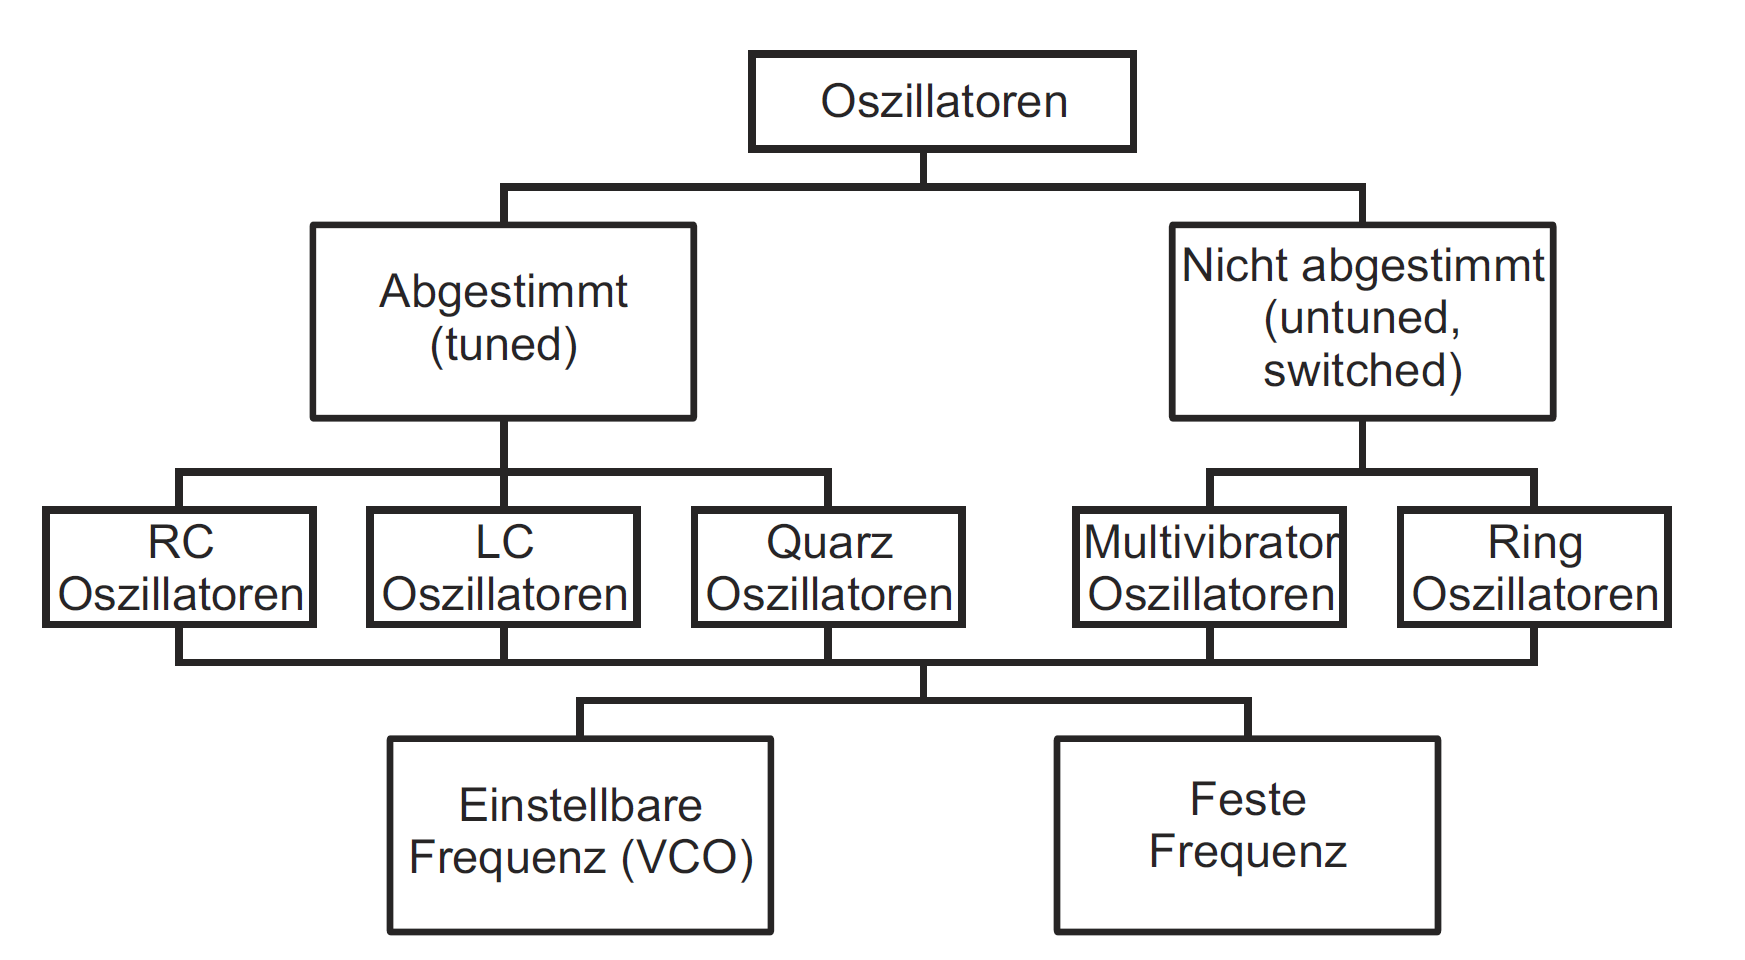
\includegraphics[width=11cm]{images/osziTypen.png}
	\end{center}

\subsection{Untuned Oscillators}
	\subsubsection{Astabiler Multivibrator mit Transistor}
	\begin{minipage}{6cm}
		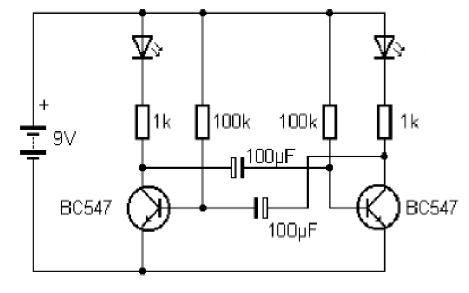
\includegraphics[width=6cm]{images/multiVibrator}
	\end{minipage}
	\begin{minipage}{10cm}
		$t_1 = t_2 = 0.7 \cdot 100k\Omega \cdot 100\mu F$ \\
		$T = t_1 + t_2$
	\end{minipage}

\subsubsection{Astabiler Multivibrator mit Komparator}
	\begin{multicols}{3}
		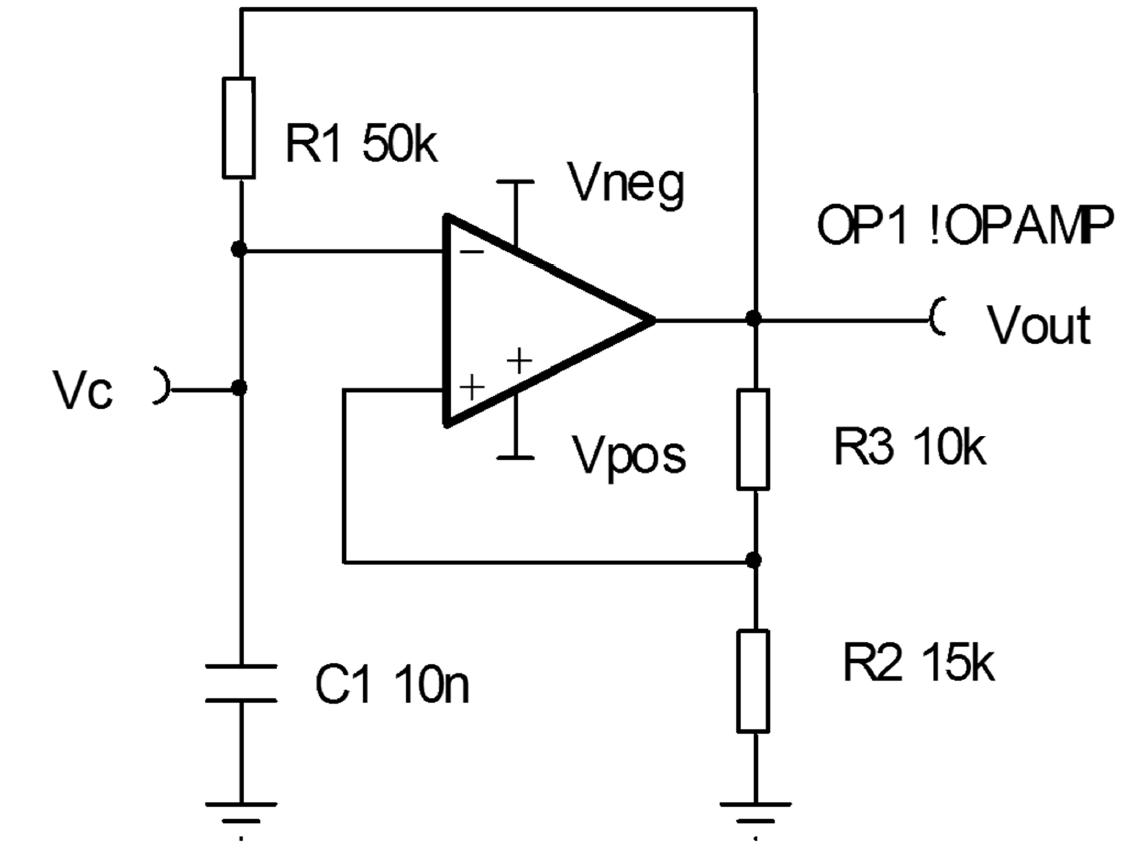
\includegraphics[width=6cm]{images/osziRechteck.png}
		\columnbreak
		
		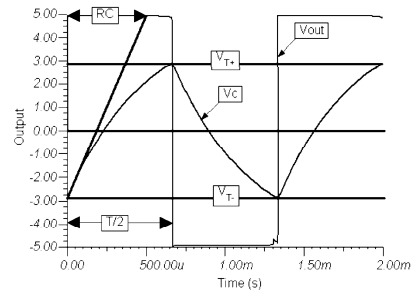
\includegraphics[width=6cm]{images/osziRechteckSignal.png}
		\columnbreak
		
		$V_{T+}=V_{outMAX}\cdot\frac{R_2}{R_2+R_3}$\\
		$V_{T-}=V_{outMIN}\cdot\frac{R_2}{R_2+R_3}$\\
		$V_c(t)=V_{T-}+\left(V_{outMAX}-V_{T-}\right)\left(1-e^{\frac{-t}{R_1\cdot
		C_1}}\right)$\\
		$f=\frac{1}{T}=\frac{1}{2R_1C_1 ln \frac{R_3+2R_2}{R3}}$\\
		wenn: $R2 = 0.86 \cdot R_3$ dann gilt:\\
		$f=\frac{1}{2\cdot R_1C_1}$
	\end{multicols}
\subsubsection{Dreieck Rechteck Generator}
	\begin{multicols}{3}
		\begin{center}
			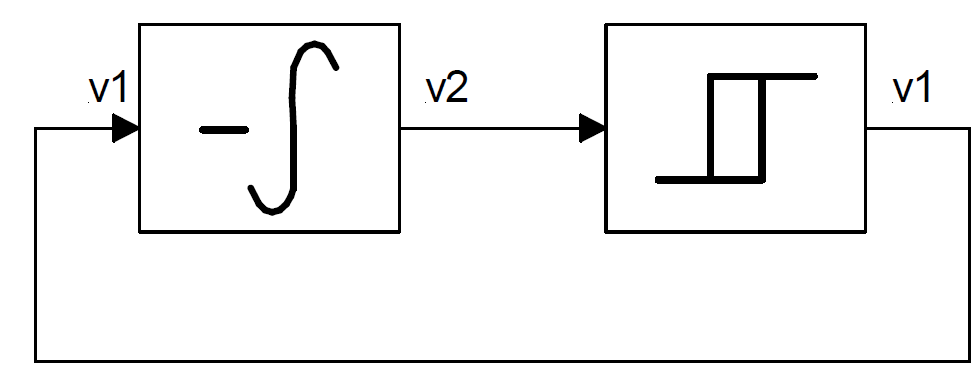
\includegraphics[width=3.5cm]{images/osziDreieckRechteckBlock.png}\\
		\end{center}
		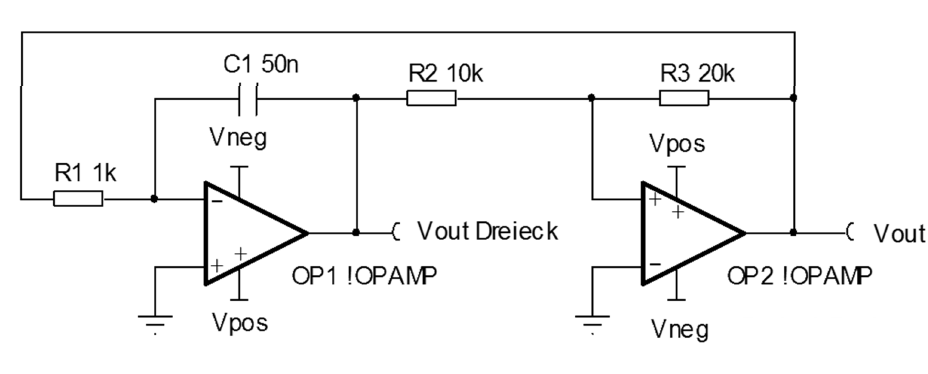
\includegraphics[width=6cm]{images/osziDreieckRechteck.png}
		\columnbreak
		
		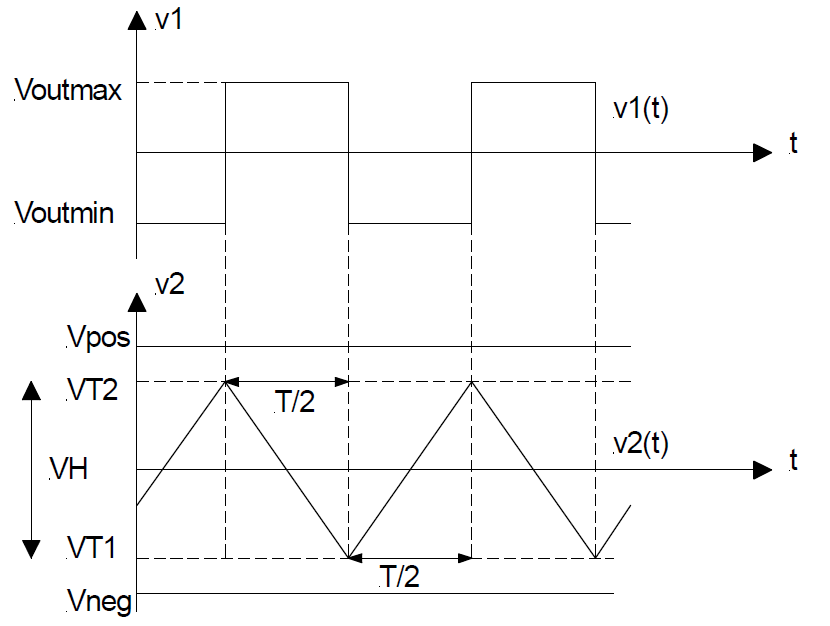
\includegraphics[width=6cm]{images/osziDreieckRechteckSignal.png}
		\columnbreak
			
		$V_2\left(t\right)=-\frac{1}{R_1C}\int V_1\left(t\right)dt+V_{2 Anfang}$\\
		$V_H=2\left|V_T\right|=\left(V_{outMAX}-V_{outMIN}\right)\frac{R_2}{R_3}$\\
		$T=\frac{2\cot V_H \cdot R_1C}{V_{outMAX}}$\\
	\end{multicols}
\subsubsection{Kippschaltung}
	\begin{minipage}{9cm}
		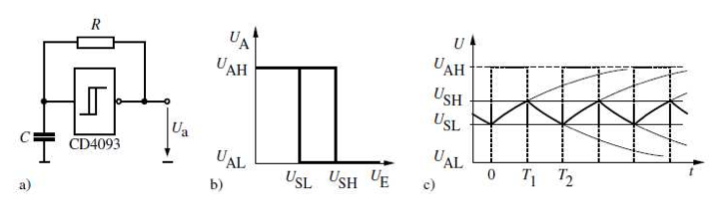
\includegraphics[width=9cm]{images/kippschaltung}
	\end{minipage}
	\begin{minipage}{6cm}
		$\tau = R \cdot C $\\
		$T_1 = \tau \cdot \ln \left(\frac{U_{AH}-U_{SL}}{U_{AH}-U_{SH}} \right)$ \\
		$T_2 = \tau \cdot \ln \left(\frac{U_{SH}-U_{AL}}{U_{SL}-U_{AL}} \right)$ \\
		$f = \frac{1}{T_1 + T_2}$
	\end{minipage}
\subsubsection{Ringoszilatoren}
	\begin{minipage}[T]{6cm}
		Schaltung mit Invertern: \\
		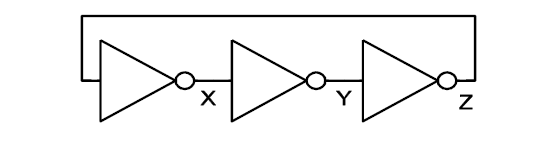
\includegraphics[width=6cm]{images/osziRing.png} \\
		\[ f_{osc} = \frac{1}{2 \cdot n \cdot t_g} \] 
	\end{minipage}
	\begin{minipage}{6cm}
		Schaltung mit MOS-FETs: \\
		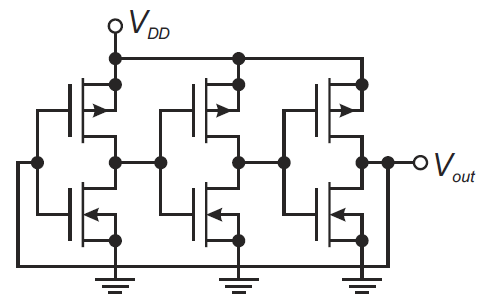
\includegraphics[width=6cm]{images/osziRingCMOS.png} \\
	\end{minipage}
	\begin{minipage}{6cm}
		Zeitliches Verhalten: \\
		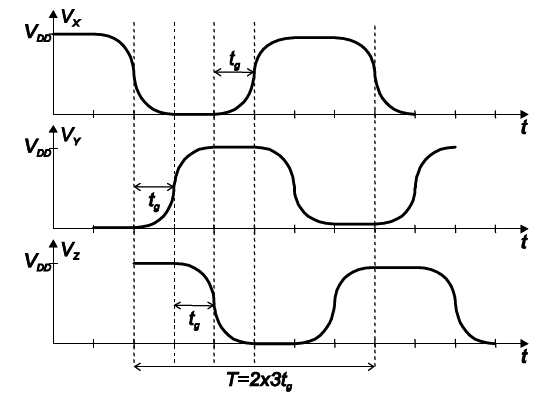
\includegraphics[width=5.5cm]{images/osziRingSignal.png} \\
	\end{minipage}	

\newpage	
\subsection{Tuned Oscillators}
	Oszillatoren mit Rückkopplung. Schwingbedingung: Verstärkung im gesamten Kreis $=1$. 
	\subsubsection{LC-Oszillator}
		\begin{multicols}{2}
		
			\textbf{Normaler LC-Oszillator} \\
			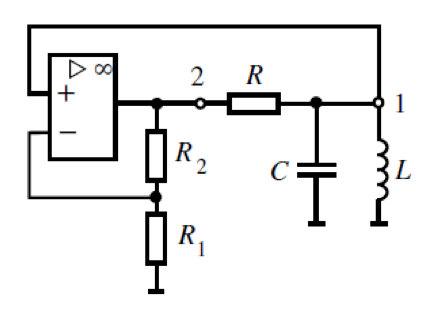
\includegraphics[width=6cm]{images/lcOszillator} 
			
			\begin{multline*}	
				U_2(t) = (1+\frac{R_2}{R_1}) \cdot U_1(t) = V_u \cdot U_1(t) \\
				\text{Daraus folgt die Schwingungsgleichung:} \\
				\frac{d^2 U_1(t)}{dt^2}+2k\omega_0 \frac{dU_1(t)}{dt}+\omega^2U_1(t)=0 \\
				\text{und somit } \omega_0 = \frac{1}{\sqrt{L\cdot C}} \\
			\end{multline*}
			
		\columnbreak
		
			\textbf{Colpitts-Oszillator} \\
			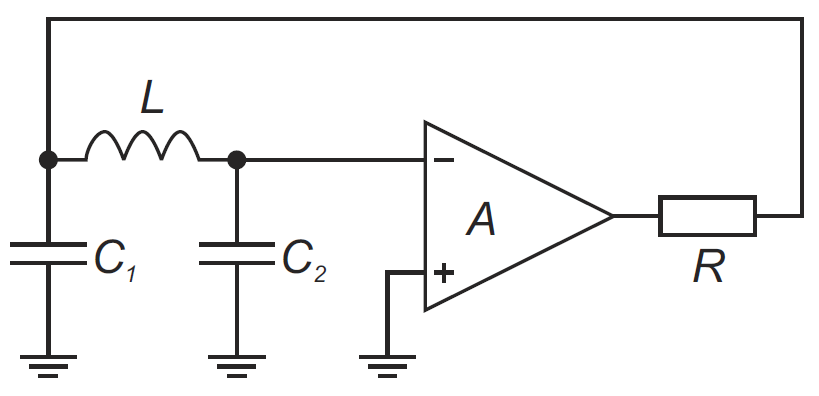
\includegraphics[width=7cm]{images/osziLC.png} \\
		
			\[ \omega_0=\frac{1}{\sqrt{L\frac{C_1 C_2}{C_1+C_2}}} \] \\
		\end{multicols}

	\subsubsection{Quarz-Oszilator}
		\begin{tabular}{lll}
			\textbf{Ersatzschaltung} & \textbf{Phasengang} & \textbf{Anwendung} \\
			\begin{minipage}{6cm}
				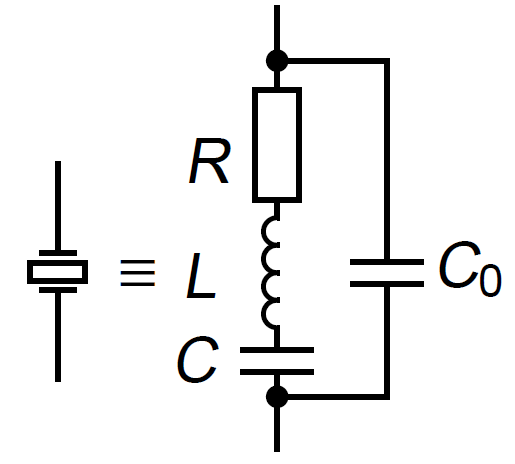
\includegraphics[width=3cm]{images/osziCrystal.png}
			\end{minipage} &
			\begin{minipage}{6cm}
				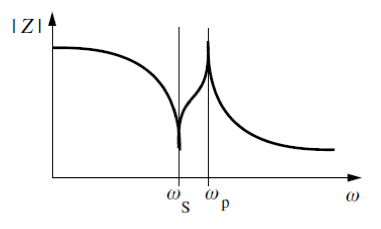
\includegraphics[width=5cm]{images/quarz-kennl.png}
			\end{minipage} & 
			\begin{minipage}{6cm}
					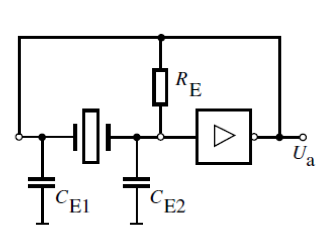
\includegraphics[width=5cm]{images/quarz-schaltung.png}
			\end{minipage}	\\
		\end{tabular}	
			
		Frequenzabweichung: $\frac{\Delta f}{f_0} \approx 10^{-6} \dots 10^{-10}$ \\
		
	\subsection{Spannungsgesteuerte Oszillatoren (VCO)}
		\begin{minipage}{12cm}
			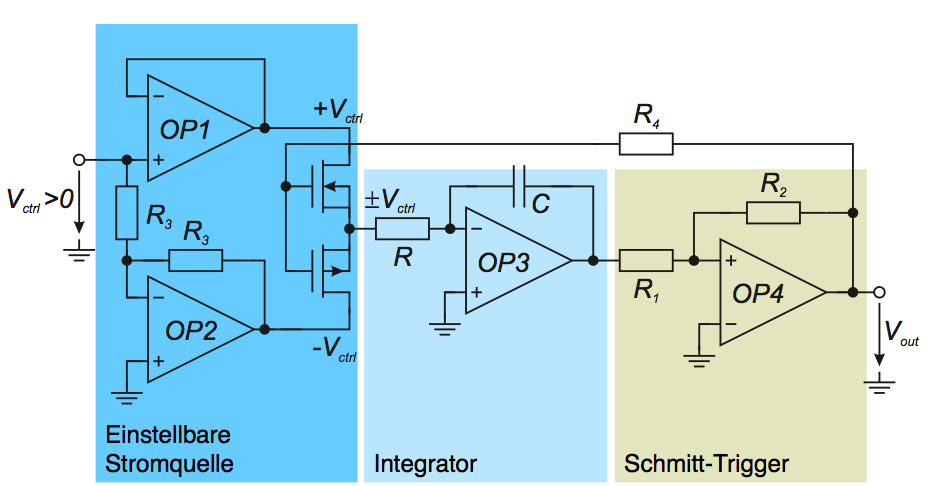
\includegraphics[width=12cm]{images/vco.png}
		\end{minipage}
		\begin{minipage}{6cm}
			$f_{osc} = \frac{R_1 + R_2}{4 R_1} \cdot \frac{1}{RC} \cdot \frac{U_{ctrl}}{|U_{out}|}$ \\
			
			was vereinfacht wird zu \\
			$f_{osc} = K_{VCO} \cdot U_{ctrl}$ mit $K_{VCO}$ als konstantem Faktor.
		\end{minipage}